\vspace*{-1mm}
In Chapter~\ref{Ch:CC_noise_theory} the theoretical model (Mastoridis--Baudrenghien model) for the transverse emittance growth caused by amplitude and phase noise in a $\CC$ was discussed. On September 5, 2018, a dedicated experiment was conducted in the SPS to benchmark this model against experimental data and confirm the analytical predictions. In particular, the aim was to inject artificial noise into the $\CC$ RF system and compare the measured emittance growth rates with the theoretically computed ones. In this chapter, the measurement results from the SPS are presented and discussed. However, since a similar experiment has not been performed before, this chapter does not present only the emittance growth measurements. It also discusses in detail the experimental conditions and the available measurements of other parameters of interest such as the $\CC$ voltage, the RF noise sepctra, the bunch length, and the bunch intensity, aiming to provide a full understanding
%The work published in Ref.~\cite{Triantafyllou:2021khx} is the basis of this chapter.


Section~\ref{sec:CCs_sps_details} provides some information on the installation of the $\CC$s in the SPS that are essential for the studies in this thesis and elaborates on some considerations regarding their operation in the SPS. Afterward, Section~\ref{sec:exp_setup_2018} describes the machine setup and the beam configuration for the emittance growth measurements. This includes a summary of the preparatory studies conducted in the previous years. In Section~\ref{sec:injected_RF_noise} information on the noise injected in the $\CC$ RF system is provided while in Section~\ref{subsec:CC_voltage_2018_measurement} the beam-based measurement of the $\CC$ voltage is presented. The measurements of transverse emittance growth are presented in Section~\ref{sec:emit_growth_meas_2018} while the complementary measurements of bunch length and intensity in Section~\ref{sec:bunch_length_intensity_meas_2018}. Section~\ref{sec:meas_2018_vs_theory} compares the measured transverse emittance growth against the predictions of Mastoridis--Baudrenghien model. The conclusions of the first experimental campaign with $\CC$ noise in SPS are drawn in Section~\ref{sec:MD2018_conclusions}.

\section{Crab Cavities in the SPS}\label{sec:CCs_sps_details}
For the SPS tests of 2018 two prototype $\CC$s of the Double Quarter Wave (DQW) type \footnote{The RFD type $\CC$s are expected to be ready by the end of 2022 - beginning of 2023.}, which will be referred to as $\CC$1 and $\CC2$ throught this thesis, were fabricated by CERN and were assembled in the same cryomodule. %, shown in Fig.~\ref{fig:DQW_cryomodule}~\cite{Zanoni:2017}.
For its installation an available space was found at the SPS Long Straight Section 6 (SPS-LSS6) zone. As this section is also used for the extraction of the beam to the LHC, the cryomodule was placed on a mobile transfer table~\cite{Calaga:2649807} which  moved the cryomodule in the beamline for the $\CC$ tests and out of it for the usual SPS operation without breaking the vaccum.
 
 The main $\CC$s' parameters are listed in Table~\ref{tab:SPS_CC_main}. Their location along the SPS ring is also indicated, in case someone would like to repeat the analysis described in this thesis.

 \begin{table}[!hbt]
    \begin{minipage}{\textwidth}
    %\centering
    \begin{centering}
    \caption{Crab Cavities design parameters for the SPS tests.}
    \begin{tabu} to \textwidth {X[c,0.1m] X[c,m] X[0.5c,m] X[0.5c,m]}
       &&& \\[-6mm]
       \toprule \toprule
       \multicolumn{2}{l}{\textbf{Parameter}} &
       \multicolumn{2}{c}{\textbf{Value}} \\
       \bottomrule
       \multicolumn{2}{l}{} & 	\multicolumn{1}{c}{\textbf{CC1}} & \multicolumn{1}{c}{\textbf{CC2}} \\
       \midrule
       \multicolumn{2}{l}{crabbing plane}  & \multicolumn{1}{c}{vertical} & \multicolumn{1}{c}{vertical} \\
       
       \multicolumn{2}{l}{s-location$^{\ast}$}  & \multicolumn{1}{c}{6312.72\,m} & \multicolumn{1}{c}{6313.32\,m} \\
 
       \multicolumn{2}{l}{$\CC$ voltage, $\CCvoltage$}  & \multicolumn{1}{c}{$\leq$ 3.4\,MV} & \multicolumn{1}{c}{$\leq$ 3.4\,MV} \\
 
       \multicolumn{2}{l}{$\CC$ frequency, $\CCvoltage$}  & \multicolumn{1}{c}{400.78\,MHz} & \multicolumn{1}{c}{400.78\,MHz} \\ %400.789
 
       \multicolumn{2}{l}{Horizontal / Vertical beta function, $\beta_{x, CC}$ / $\beta_{y, CC}$}  & \multicolumn{1}{c}{29.24\,m / 76.07\,m} & \multicolumn{1}{c}{30.31\,m / 73.82\,m} \\
 
       \multicolumn{2}{l}{Horizontal / Vertical alpha function, $\alpha_{x, CC}$ / $\alpha_{y, CC}$} & \multicolumn{1}{c}{-0.88\,m / 1.9\,m} & \multicolumn{1}{c}{-0.91\,m / 1.86\,m} \\
 
       \multicolumn{2}{l}{Horizontal / Vertical dispersion, $D_{x, CC}$ / $D_{y, CC}$} & \multicolumn{1}{c}{-0.48\,m / 0\,m}  & \multicolumn{1}{c}{-0.5\,m / 0\,m} \\
       \arrayrulecolor{black}\bottomrule
    \end{tabu}
    \label{tab:SPS_CC_main}
    \end{centering} \footnotesize{$^\ast$ The s-location is reffered to the location of the elements along the SPS ring with respect to the start of the lattice i.e. element QF.10010 which is a focusing quadrupole. The s-location is given to allow the studies to be reproduced.}
    \end{minipage}
 \end{table}
 % QF.10010  is the start of the SPS lattice --> https://layout.cern.ch/reports/mad?fileType=STANDARD&machineId=2180065&versionId=34464591 (access with sshuttle)
 % The actual start of the lattice at 0 m is: %BEGI.10010. which is a marker (not a real element).
 
 % Optics parameters for CC and diagnostics in 2018: https://cernbox.cern.ch/index.php/apps/files/?dir=/__myshares/SPS_MDs_2018%20(id%3A271128)/SPSMeasurementTools&#editor
 
 \subsection{Considerations about the Crab Cavity operation}\label{sec:cc_setup}
The experimental studies presented in this thesis, were performed with the $\CC$s operating at a fixed frequency of 400.78\,MHz (unless it is stated otherwise) and at a target peak voltage of about 1\,MV. % this is for 270 GeV.
Even though the $\CC$ modules installed in the SPS can operate at a maximum voltage of 3.4\,MV (see Table~\ref{tab:SPS_CC_main}), the experiments were performed with peak voltage of 1\,MV since for that value the stable $\CC$ operation for long periods was ensured. Further details on the hardware aspects of the $\CC$ operation in the SPS are not discussed here as they are out of the scope of this thesis.

\normalsize{\textbf{Energy ramp}}\\
SPS receives the proton beam at 26\,GeV from the PS. It was found that the ramp to higher energies could not be performed with the $\CC$ switched on, since during the acceleration one of the vertical betatron sidebands was crossing the $\CC$ frequecny resulting to resonance excitation and beam loss~\cite{BE_seminar, CC_rephasing_RF}. Changing the $\CC$ frequnecy during the ramp so that it stays synchronous with the beam was not an option due to hardware limitations~\cite{CC_rephasing_RF}. % CC not fast enough.
Therefore, it was established that the acceleration has to be performed with the $\CC$ switched off and its voltage must be set up only after the energy of interest has been achieved. It is worth noting that this approach will also be used in the HL-LHC.
%while crossing one of the vertical betatron sidebands due to resonant excitation~\cite{BE_seminar, CC_rephasing_RF}. Therefore, it was established that the acceleration has to be performed with the $\CC$ switched off and its voltage must be set up only after the energy of interest has been achieved. It is worth noting that this approach will also be used in the HL-LHC.

\normalsize{\textbf{Crab Cavity - main SPS RF synchronisation}}\\
In order to ensure that the beam will experience the same kick from the $\CC$ each turn the SPS main RF system operating at $\sim$200\,MHz needed to be synchronous with the $\CC$ operating at 400.78\,MHz. Due to the larger bandwidth of the SPS main RF system the $\CC$ was used as a master. Therefore the $\CC$ was operating at a fixed frequency, while the main accelerating cavities were adjusted to the exact half of the $\CC$ frequency so that they become synchronous with the crabbing signal. For studies at higher energies the synchronisation took place at the end of the energy ramp shortly a few seconds after the $\CC$ was switched on~\cite{BE_seminar}. %(refer to Fig.~\ref{fig:sps_cycles_cc_tests} for the parts of the acceleration cycle). 


%It was important to ensure that during the "coast" the beam will experience the same kick from the $\CC$ each turn.


\section{Experimental configuration and procedure}\label{sec:exp_setup_2018}
This section gives an overview of the experimental setup and the procedure that was followed. First, it briefly discusses the preparatory studies that were performed during 2012-2017~\cite{Calaga:1451286, Alekou_CC_coast_prep_2016, Antoniou:2649815}, explaining the choice of the intensity and energy values for which the emittance growth measurements were conducted. Furthermore, it presents in detail the rest of the beam and machine conditions during the experiment. Last, the experimental procedure is explained.

%\normalsize{\textbf{Preparatory experimental studies}}\\
\subsection{Preparatory experimental studies}\label{sec:preparatory_studies_for_2018_MD}
For studying the long-term emittance evolution a special mode of operation was set up in the SPS which is called "coast" (in other machines, it is referred to as storage ring mode) with bunched beams. In this mode, the bunches circulate in the machine at constant energy for long periods, from a few minutes up to several hours, similar to the HL-LHC case.\setlength{\parskip}{2ex} %set it manually here, as for some reason it was not displayed properly in the pdf.

To make sure that the SPS can be used as a testbed for the emittance growth studies with $\CC$s an extensive preparatory campaign was carried out through 2012-2017~\cite{Calaga:1451286, Alekou_CC_coast_prep_2016, Antoniou:2649815}. The primary concern was the emittance growth that was observed in the machine from other sources than injected noise and will be referred to as the natural emittance growth in this thesis. The natural emittance growth needs to be well characterised and be kept sufficiently small in order to distinguish and understand the contribution from the $\CC$ noise. 

From these studies, it was concluded that the optimal coast setup is at high energies, with low chromaticity and bunches of low intensity as it minimises the natural emittance growth~\cite{Antoniou:2649815}. The highest energy for which the SPS could operate in coast was 270\,GeV and thus the experiments were performed at this energy.  That limitation was introduced due to limited cooling of the magnets to transfer away the heating when operating at high energy and thus at large currents for long periods. %heating of the magnets from large current in the coils, when operating at high energy for long periods. 
Moreover, as the natural emittance growth was found to be a single bunch effect four bunches were used. That choice was made to reduce the statistical uncertainty of the measurements but not to increase the beam intensity.




%\normalsize{\textbf{Machine and beam configuration}}\\
\subsection{Machine and beam configuration}
During the experiment the Landau octupoles were switched off. Nevetherless, a residual non-linearity was present in the machine mainly due to multipole components in the dipole magnets~\cite{Carlà:2664976, Alekou:2640326}. The transverse feedback system was also switched off. Unfortunately, no measurements of chromaticity are available from the day of the experiment. However it was ensured that the chromaticity was corrected to small positive values. Last, only one $\CC$, $\CC 2$, was used for simplicity and it operated at 1\,MV.

The main machine and beam parameters used for the emittance growth measurements in 2018 are listed in Table~\ref{tab:machine_beam_param_2018}. % the parameters shown are the relatives one for Eq.(3.1) and (3.2) --> theoretical formulas for the emittance growht.


\begin{table}[!hbt]
	\begin{minipage}{\textwidth}
      \begin{centering}
   \caption{Main machine and beam parameters for the emittance growth studies with CCs in SPS in 2018.}
	\begin{tabu} to \textwidth {X[c,m] X[0.5c,m] X[0.5c,m] X[0.01c,m]}
		&&& \\[-6mm]
		\toprule \toprule
		\multicolumn{2}{l}{\textbf{Parameter}} &
		\multicolumn{2}{c}{\textbf{Value}} \\
		\bottomrule
      \multicolumn{2}{l}{Beam energy, $\symE$} & \multicolumn{2}{c}{270\,GeV} \\
      \multicolumn{2}{l}{Revolution frequency, $\frev$}  & \multicolumn{2}{c}{43.375\,kHz} \\
      \multicolumn{2}{l}{Main RF voltage / frequency,  $\VRF$ / $\fRF$}  & \multicolumn{2}{c}{3.8\,MV / 200.39\,MHz} \\ %200.3945
      \multicolumn{2}{l}{Horizontal / Vertical betatron tune, $\Qx$ / $\Qy$}  & \multicolumn{2}{c}{26.13 / 26.18} \\
      \multicolumn{2}{l}{Horizontal / Vertical first order chromaticity, $\Qpx$ / $\Qpy$}  & \multicolumn{2}{c}{ $\sim$ 1.0 / $\sim$ 1.0} \\
      \multicolumn{2}{l}{Synchrotron tune, $\Qs$}  & \multicolumn{2}{c}{0.0051} \\
      \multicolumn{2}{l}{$\CC 2$ voltage / frequency, $\CCvoltage$ / $\CCfrequency$}  & \multicolumn{2}{c}{1\,MV / 400.78\,MHz} \\
      \multicolumn{2}{l}{Number of protons per bunch, $\Nb$} & \multicolumn{2}{c}{3 $\times 10^{10}$ p/b$^\ast$} \\
      \multicolumn{2}{l}{Number of bunches}  & \multicolumn{2}{c}{4} \\
      \multicolumn{2}{l}{Bunch spacing}  & \multicolumn{2}{c}{524\,ns} \\
      \multicolumn{2}{l}{Rms bunch length, 4$\sigmat$}  & \multicolumn{2}{c}{1.8 \,ns$^\ast$}\\
      \multicolumn{2}{l}{Horizontal / Vertical normalised emittance, $\emitx$ / $\emity$}  & \multicolumn{2}{c}{2\,$\mathrm{\mu m}$ / 2\,$\mathrm{\mu m^\ast}$}\\
      \multicolumn{2}{l}{Horizontal / Vertical rms tune spread, $\Dqxrms$ / $\Dqyrms$}  & \multicolumn{2}{c}{2.02 $\times 10^{-5}$ / 2.17 $\times 10^{-5}$ $^\dagger$}\\
      \bottomrule
	\end{tabu}
   \label{tab:machine_beam_param_2018}
   \end{centering} \footnotesize{$^\ast$ The value corresponds to the requested intial value at the start of each coast. The measured evolution of the parameter through the experiment is presented in the Sections~\ref{sec:emit_growth_meas_2018} and~\ref{sec:bunch_length_intensity_meas_2018}.\\$^\dagger$ Here the rms betatron tune spread includes only the contribution from the detuning with amplitude present in the SPS machine. The calulcations for the listed values can be found in Appendix~\ref{app:detuning_with_amplitude}.}
   \end{minipage}
\end{table}


%\normalsize{\textbf{Experimental procedure}}\\
\subsection{Experimental procedure for emittance growth measurements}\label{sec:experimental_procedure_2018}
The emittance growth experiment took place on September 5, 2018, and was given a total time window of about 6 hours (start:$\sim$10:30, end:$\sim$17:00). In order to characterize the CC noise induced emittance growth, different levels of controlled noise were injected into the low-level RF system and the bunch evolution was recorded for about 20-40 minutes (for each noise setting). The experiment was conducted over three coasts, since a new beam was injected every time the quality of the beam was seen to be degraded e.g. very large beam size. In the following, the different noise settings will be denoted as "Coast$N$-Setting$M$", where $N$ stands for the coast number and $M$ for the different noise levels applied in each coast in chronological order. After the experiment, the measured growth rates would be compared with the theoretically expected values from the model described in Chapter~\ref{Ch:CC_noise_theory}.
%The dedicated experiment to study the emittance growth induced by noise in the $\CC$ RF sytsem took place on September 5, 2018, and was given a total time window of about 16 hours (start:$\sim$10:30, end:$\sim$17:00).

\section{Injected RF noise}\label{sec:injected_RF_noise}
The noise injected in the $\CC$ RF system was a mixture of amplitude and phase noise up to 10\,kHz, overlapping and primarily exciting the first betatron sideband at $\sim 7.8$\,kHz (see discussion in Section~\ref{subsec:CC_emit_growth_theoretical_formulas}). The phase noise was always dominant. The noise levels were measured with a spectrum analyzer E5052B~\cite{E5052B_insight} and are expressed as $10\log_{10}\mathcal{L}(f)$\,[dBc/Hz]. The relation between the measured noise levels and the power spectral densities in Eq.~\eqref{eq:dey_an} and Eq.~\eqref{eq:dey_pn} is given by $S_\Delta = 2\mathcal{L}(f)$, with $S_{\Delta A}$ in\,Hz$^{-1}$ and $S_{\Delta \phi}$ in $\mathrm{rad^2 Hz^{-1}}$. This relation is extensively discussed in Appendix~\ref{ch:app_B} and specifically in~\ref{app:Measured_noise}}. Figure~\ref{fig:example_PN_and_AN_coast1_setting2} displays an example measurement of amplitude (left) and phase (right) noise acquired during the experiment.

 % Loaction for creating the figure: /eos/user/n/natriant/2018/CC_MD_2018_summary/measured_psd/for_thesis/
 \begin{figure}[!ht]
   \centering
   \begin{subfigure}[t]{0.45\textwidth}
       \centering
       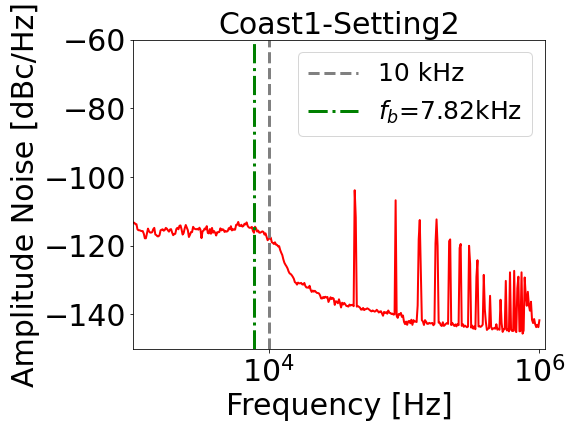
\includegraphics[width=1\textwidth]{images/Ch5/Measured_spectrum_MD5_Coast1-Setting2-AN.csv_no_psd.png}
       %\caption{$y=\sin(2 \pi f t),\ f=50$ Hz}
       %\label{fig:add_label_here}
   \end{subfigure}
   \hfill
   \begin{subfigure}[t]{0.45\textwidth}
       \centering
       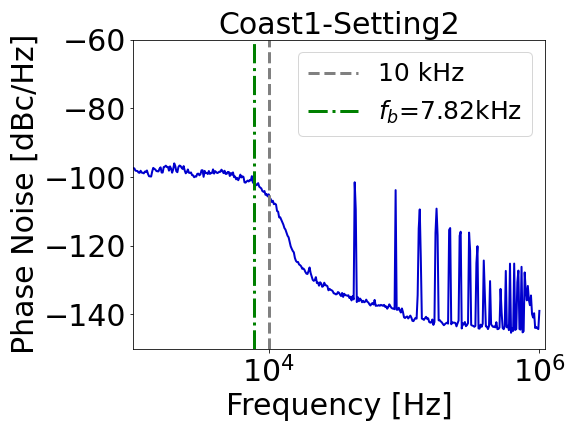
\includegraphics[width=1\textwidth]{images/Ch5/Measured_spectrum_MD5_Coast1-Setting2-PN.csv_no_psd.png}
       %\caption{Discrete Fourier transform}
       %\label{fig:add_label_here}
   \end{subfigure}
   \hfill
    \caption{Example amplitude (left) and phase (right) noise spectra measured with a spectrum analyzer E5052B~\cite{E5052B_insight} during the emittance growth studies with CCs in SPS. The noise extends up to 10\,kHz (grey dashed line) overlapping the first betatron sideband at $\sim$8\,kHz (green dashed line). The spikes at high frequencies correspond to the harmonics of the revolution frequency and are a result of the beam induced signal from its passage through the CC.} % bunch passage
    \label{fig:example_PN_and_AN_coast1_setting2}
\end{figure}

The spectrum analyzer E5052B~\cite{E5052B_insight},  was directly attached to the RF antenna inside the $\CC$ which monitors the amplitude and the phase of its field. To this end, the voltage induced by the passage of the bunch through the $\CC$ was visible in the measured spectra: spikes at high frequencies and in particular at harmonics of the revolution frequency.
% RF pick up anterna of CC: https://www.osti.gov/servlets/purl/1542783

% the bunch passes through the cc and it induces its own voltage. It is captured by the antenna as spikes in the frequency spectrum.

\subsubsection*{Power spectral density values of interest}
As already discussed in Chapter~\ref{Ch:CC_noise_theory} the noise induced emittance growth depends on the noise power at the betatron and synchrobetatron sidebands for the phase and amplitude noise respectively (see Eq.~\eqref{eq:dey_pn} and Eq.~\eqref{eq:dey_an}). Therefore, the noise power values of interest for this thesis are the ones at the first betatron $f_b = 0.18 \times \frev$ = 7.82\,kHz and at the synchrobetatron sidebands at $f_b \pm \Qs \times \frev  = f_b \pm  \sim 220$\,kHz (see discussion in Section~\ref{subsec:CC_emit_growth_theoretical_formulas}).


However, it can be clearly seen from Fig.~\ref{fig:example_PN_and_AN_coast1_setting2} that the measured noise spectra are noisy\footnote{This is not surprising since it is in the nature of the noise.}: random changes in amplitude are observed from point to point within the signal. 
To get a more precise value of the power sepctral density value at the first betatron sideband, $f_b$, the average of the power spectral density values over a frequency range of $\pm$ 500\,Hz around it is considered while its uncertainty equals the standard deviation over that range. In the following, it is also assumed for simplicity that the noise power between the synchrobetatron sidebands and the first betaton sideband is smooth as they lie very close to each other. This means that the power spectral density at the synchrobetatron sidebands equals the power spectral density at the first betaton sideband.

%is determined as the average of the power spectral density values over a frequency range of $\pm$ 500\,Hz around it, while its uncertainty is considered to be the standard deviation over that range. In the following, it is assumed for simplicity that the power spectral density at the synchrobetatron sidebands equals the power spectral density at the first betaton sideband as they lie very close to each other. %At this point, it should be mentioned that the validity of these assumptions was tested with numerical simulations which used the measured spectra (Chapter~\ref{Ch:investigating_discrepancy}).

The emittance growth measurements were performed with seven different noise levels. The values of the phase and amplitude noise for each setting are listed in Table~\ref{tab:noise_settings_2018}. 

\subsubsection*{Effective phase noise}
In order to make a meaningful comparison between the different levels of noise, the concept of effective phase noise is introduced: this is the phase noise level that would lead to the same emittance growth as that from both phase and amplitude noise according to the theoretical model (Chapter~\ref{Ch:CC_noise_theory}). 

For the calulcation of the effective phase noise the averaged bunch length for each case is used (bunch length measurements at Section~\ref{sec:bunch_length_intensity_meas_2018}). The uncertainty on the effective phase noise is computed following the standard procedure of the propagation of the uncertainty (Appendix~\ref{app:uncertainty_propagation}). \textcolor{red}{Do I need to show all the calulcations?.} The calculated effective phase noise values for the experimental conditions are also listed in Table~\ref{tab:noise_settings_2018}. The values shown correspond to the results using the parameters of the first bunch. However, the difference between the values for the other bunches is very small and is also within the displayed uncertainties. The noise levels mentioned in the following analysis of the experimental data correspond to the calculated effective phase noise. 
% Script for computing the values: /eos/user/n/natriant/2018/CC_MD_2018_summary/measured_psd/job001_cmpt_psd_at_fb.ipynb
% The resulted pickle file can be found at: /eos/user/n/natriant/2018/CC_MD_2018_summary/measured_psd/output
% Effective phase noise: /eos/user/n/natriant/2018/CC_MD_2018_summary/measured_psd/job002_cmpt_effective_PN.ipynb
% Analytical calculations of the effective phase noise and its uncertainty: /eos/user/n/natriant/2018/CC_MD_2018_summary/measured_psd/notes_on_computing_effective_pn_psd_and_uncertainties.pdf

\begin{table}[!hbt]
	\centering
   \caption{Phase and amplitude noise levels injected in the CC RF system for the emittance growth studies of 2018. The listed values correspond to the average power spectral density values over a frequency range of $\pm$ 500\,Hz around the first betatron sideband, $f_b$. The calculated effective phase noise for the parameters of the first bunch are also listed.}
	\begin{tabu} to \textwidth { X[c,m] X[c,m] X[c,m] X[c,m]}
		&&& \\[-6mm]
		\toprule \toprule
		\multicolumn{1}{l}{} &
		\multicolumn{3}{c}{$\mathbf{10\,\boldsymbol{\log}_{10} \mathcal{L}(f)}$ \textbf{[dBc/Hz]}} \\
		\bottomrule
      \multicolumn{1}{l}{} & 	\multicolumn{1}{c}{\textbf{Phase noise}} & \multicolumn{1}{c}{\textbf{Amplitude noise}} & 	\multicolumn{1}{c}{\textbf{Effective phase noise}} \\
      \midrule
      \multicolumn{1}{l}{Coast1-Setting1}  & \multicolumn{1}{c}{-122.6 $\pm 0.6$} & \multicolumn{1}{c}{-128.1 $\pm$ 0.6} & \multicolumn{1}{c}{-121.8 $\pm$ 0.5} \\
      
      \multicolumn{1}{l}{Coast1-Setting2}  & \multicolumn{1}{c}{-101.4 $\pm$ 0.8} & \multicolumn{1}{c}{-115.2 $\pm$ 0.6} & \multicolumn{1}{c}{-101.3 $\pm$ 0.8} \\

      \multicolumn{1}{l}{Coast2-Setting1}  & \multicolumn{1}{c}{-115.0 $\pm$ 0.8} & \multicolumn{1}{c}{-124.1 $\pm$ 0.5} & \multicolumn{1}{c}{-114.6 $\pm$ 0.7} \\

      \multicolumn{1}{l}{Coast2-Setting2}  & \multicolumn{1}{c}{-111.4 $\pm$ 0.6} & \multicolumn{1}{c}{-115.7 $\pm$ 0.4} & \multicolumn{1}{c}{-110.2 $\pm$ 0.5} \\ 

      \multicolumn{1}{l}{Coast3-Setting1}  & \multicolumn{1}{c}{-110.9 $\pm$ 0.9} & \multicolumn{1}{c}{-116.9 $\pm$ 0.4} & \multicolumn{1}{c}{-110.1 $\pm$ 0.8} \\

      \multicolumn{1}{l}{Coast3-Setting2} & \multicolumn{1}{c}{-106.4 $\pm$ 0.3} & \multicolumn{1}{c}{-112.9 $\pm$ 0.6} & \multicolumn{1}{c}{-105.8 $\pm$ 0.3}\\

      \multicolumn{1}{l}{Coast3-Setting3} & \multicolumn{1}{c}{-101.4 $\pm$ 0.7}  & \multicolumn{1}{c}{-106.9 $\pm$ 0.5} & \multicolumn{1}{c}{-100.6 $\pm$ 0.6} \\
      \arrayrulecolor{black}\bottomrule
	\end{tabu}
   \label{tab:noise_settings_2018}
\end{table}

\section{Measurement of Crab Cavity voltage}\label{subsec:CC_voltage_2018_measurement}
As mentioned above, $\CC$2 operated at 1\,MV. Before the start of the emittance growth measurements, this value was validated with beam-based measurements from the Head-Tail monitor~\cite{sps_headtail_monitor}. The Head-Tail monitor measures the transverse displacement within the bunch which can be used to reconstruct the $\CC$ voltage experienced by the beam. A detailed description of the post-processing procedure is provided in Appendix~\ref{ch:app_HT_monitor}.

The beam-based measurement of the $\CC$ voltage can only be performed right after the acceleration ramp at 270\,GeV and not during the coast mode for reasons that are explained in Appendix~\ref{ch:app_HT_monitor}. Therefore, the $\CC$ voltage was measured at the beginning of the emittance growth experiment.% before the emittance growth measurements with injected RF noise in the $\CC$. 
The $\CC$ settings remained unchanged for the rest of the experimental procedure.

The beam-based measurement of the $\CC$ voltage (reconstructed from the Head-Tail monitor) is displayed in Fig.~\ref{fig:crabbing_sin_fit_MD5} with red color. The voltage amplitude, $\CCvoltage$, is obtained from a sinusoidal fit (blue solid line in Fig.~\ref{fig:crabbing_sin_fit_MD5}) on the reconstructed voltage, $V_\mathrm{CC}(t)$, from the Head-Tail monitor reading. The standard procedure of least squares fitting (see Appendix section~\ref{app:non_linear_fitting}) is followed. In particular, $V_\mathrm{CC}(t)$ is fitted with the folllowing three-parameter ($\CCvoltage$, $\phi_\mathrm{CC}$, $d$) model function which also provides the $\CC$ phase and voltage offset:
\begin{equation}\label{eq:sin_fit_cc}
   f(x) = \CCvoltage \sin{(2\pi \CCfrequency x + \phi_\mathrm{CC})} + d ,
\end{equation}
where $\CCvoltage$ is the amplitude of the $\CC$ voltage, $ \phi_\mathrm{CC}$ the $\CC$ phase and $d$ the vertical offset of the voltage. In Eq.~\eqref{eq:sin_fit_cc} the $\CC$ frequency, $\CCfrequency$=400.78\,MHz, and is not a parameter of the fit since its operational value is fixed and well known.

%The fit is performed for a fixed $\CC$ frequency, as the operational value is fixed and well known, $\CCfrequency$=400.78\,MHz. 

% Path to plotting script: /eos/user/n/natriant/2018/CC_MD_2018_summary/2018_HT_monitor/MD5_emit_growth/plot_1example_HT_acquisition_for_thesis_5Sep2018-135033_for_thesis_sin_fit_forCh5_fixed_freq.ipynb
\begin{figure}[!h]
   \centering         
   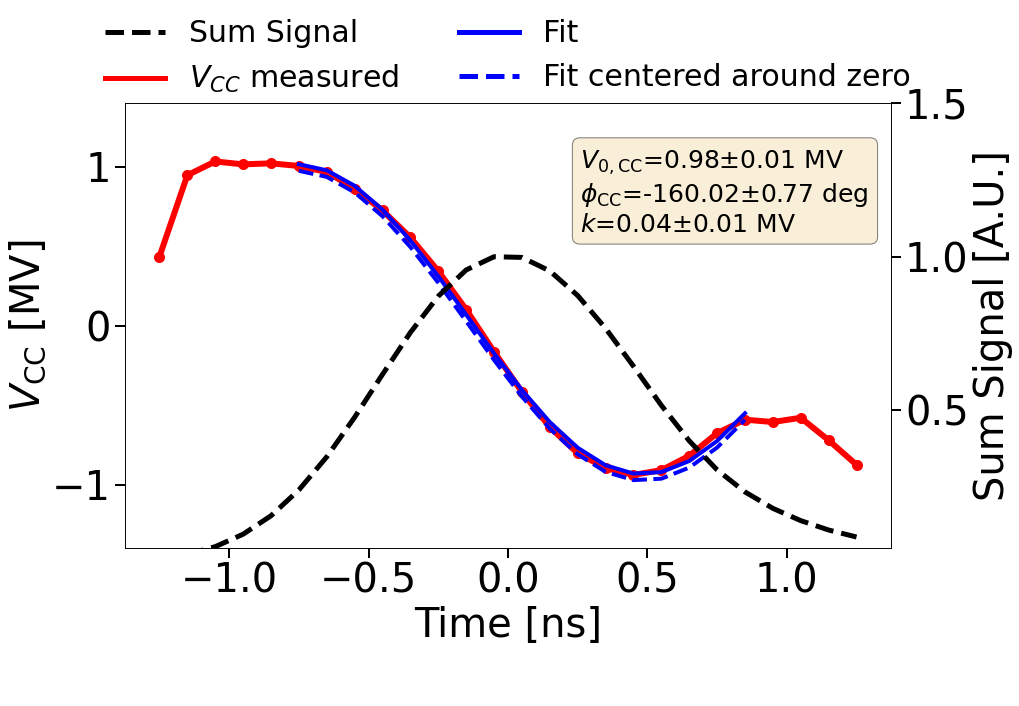
\includegraphics[width=0.7\textwidth]{images/Ch5/HT_VCC_callibration_20180905_135033_sin_fit_fixed_freq_thesis.png}
       \caption{Beam-based measurement of the CC voltage as reconstructed from the Head-Tail monitor before the emittance growth measurements in 2018 (red). The sinusoidal fit on the reconstructed voltage in order to obtain the CC voltage amplitude is also shown (blue solid line). The fit results, are given in the yellow box. The measured voltage amplitude, $V_\mathrm{0, CC}$, was found to be 0.98\,MV while its uncertainty, $d$, was measured at 0.04\,MV. The measured voltage value agrees well with the requested value of 1\,MV.}
       \label{fig:crabbing_sin_fit_MD5}
\end{figure}


The offset parameter, $d$, is added to the model function as measurements from other dedicated studies\footnote{A total of seven different dedicated experiments with $\CC$s took place in SPS in 2018 in order to address various questions on the operation of the $\CC$ with proton beams~\cite{BE_seminar}. The emittance growth experiment was the fifth in chronological order.} that took place during this first experimental campaign with $\CC$s in the SPS have shown that the reconstructed $\CC$ voltage, $V_\mathrm{CC}(t)$, is not centered around zero in the vertical axis (see Appendix Figs.~\ref{fig:VCC_from_HT_monitor_measurement} and~\ref{fig:crabbing_reconstruction_HT_monitor}). A possible explanation for the asymmetry is that it is a result of the cable response of the Head-Tail monitor pick up~\cite{Levens_WP2_HT_CC_diagnostic}. However, its origin is not yet fully understood and will have to be addressed in the future. Furthermore, it was found that the vertical offset varied between the different dedicated studies and it outweighs the error on the voltage amplitude obtained by the sinusoidal fit. To this end, in this thesis, this vertical offset $d$, will be defined as the uncertainty of the measured voltage amplitude. 
% For this topic there is a post it.

In order to obtain results that correspond to the experimental conditions the following constraints are imposed to the fit. First the voltage amplitude, $\CCvoltage$, is requested to always be positive and higher than 0.7\,MV. Furthermore, the part of the signal that corresponds to the tails of the bunch is excluded from the fit in order not to degrade its quality. Consequently, only the part of the signal for which the corresponding normalised sum signal of the Head-Tail monitor\footnote{The sum signal is the longitudinal line density. Further details are provided in Appendix~\ref{ch:app_HT_monitor}} (black dashed line) is above 0.4 is used for the fit. 

The results of the sinusoidal fit are illustrated in the yellow box in Fig.~\ref{fig:crabbing_sin_fit_MD5}. It can be concluded, that from the beam-based measurement with the Head-Tail monitor the $\CC$ voltage amplitude was found to be $\CCvoltage$=0.98$\pm$0.04\,MV. The measured value is very close to the targetd value of 1\,MV. 

\textcolor{red}{This paragraph might need to be refined.}
It is worth commenting that, the phase offset of the $\CC$ was found to be about -160$^\circ$. This means, that the $\CC$ was operating at opposite polarity than the nominal (see Eq.~\eqref{eq:CC_voltage_t}) which is also visible from the reconstructed $V_\mathrm{CC}(t)$ in Fig.~\ref{fig:crabbing_sin_fit_MD5}. The opposite polarity does not affect the emittance growth measurements. To this end the actual phase offset was measured to be $\sim 180^\circ-160^\circ=20^\circ$. This was not known during the measurement as the above mentioned analysis was performed at a later time and hence the phase offset could not be corrected. Nevertheless, simulation studies performed with Sixtracklib have shown that for the long bunches ($\sigma_z \sim$14\,cm) that were used in the for the tests in 2018, the phase offset of the $\CC$ has no significant impact on the phase noise\footnote{It is reminded here that for the emittance growth experiments the CC RF phase noise was always dominant.} induced emittance growth~\cite{wp4_triantafyllou_2020}. % slide 35 
% sin(np.pi-theta) = sin(theta)

The procedure of measuring the voltage amplitude from the Headt-Tail monitor reading and calibrating the phase offset was optimised and automated, so that it can be perfomed during the measurement, for the experimental campaigns that took place in 2022 (see Chapter~\ref{subsec:cc_calibration_2022}). 

\section{Emittance growth measurments}\label{sec:emit_growth_meas_2018}
This section presents the transverse emittance growth measurements with $\CC$ RF noise. It discusses first the measurement of the beam emittance with the SPS Wire Scanners (WS) and then it provides an overview of the emittance growth measurements for the four bunches over all the different noise settings.

\subsection{SPS Wire Scanners}\label{subsec:sps_ws}
The SPS is equipped with wire scanners (WS) to measure the transverse beam emittance. The SPS Wire Scanner system is described in detail in Ref.~\cite{BOSSER1985475, Berrig:1972478}. For the SPS tests in 2018, the emittance was measured with Wire Scanners both for the horizontal and vertical plane (BWS.51995.H and BWS.41677.V respectively).

The working principle is shown in Fig.~\ref{fig:SPS_WS_ROT}. A thin wire rapidly moves across the proton beam and a shower of secondary particles is generated. The signal from the secondary particles is then detected by a system of scintillator and photomultiplier (PM) detectors outside of the beam pipe. By measuring the photomultiplier current as a function of wire position over multiple turns the transverse beam profile is reconstructed. An example of a vertical profile is shown in Fig.~\ref{fig:WS_example_V_profile}.

\begin{figure}[!h]
   \centering         
   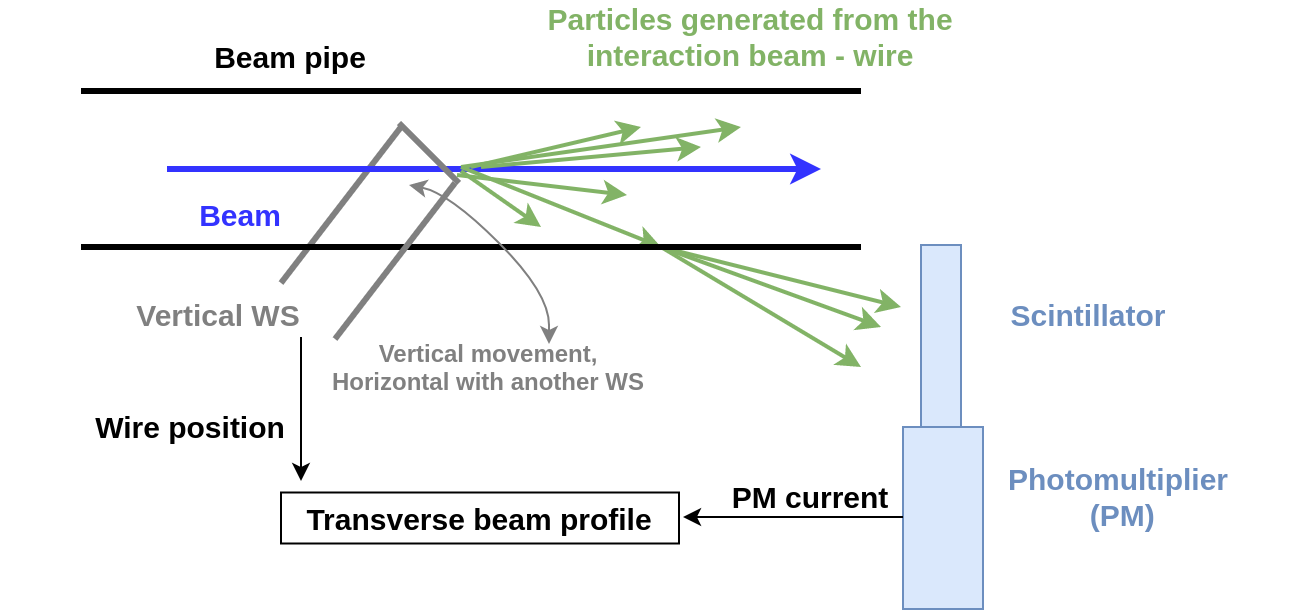
\includegraphics[width=0.8\textwidth]{images/Ch5/Wire_scanner.png}
       \caption{Sketch of the SPS rotational wire scanners~\cite{Berrig:1972478}. The wire moves across the proton beam generating secondary particles which are then detecting by a scintillator and a photomultiplier. From the measured photomultiplier current the beam profile is reconstructed.}
       \label{fig:SPS_WS_ROT}
\end{figure}
%\normalsize{\textbf{Fitting of transverse profiles}}\\
\subsubsection*{Fitting of transverse profiles}
Assuming gaussian beams and for $u=x,y$ being the index that respectively corresponds to the horizontal and vertical plane, the rms beam size, $\sigma_u$, is obtained following the standard procedure of least squares fitting (see Appendix~\ref{app:non_linear_fitting}). In particular, the measured beam profiles from each scan are fitted with the following four-parameter ($A, k, \mu, \sigma_u$) gaussian function:
\begin{equation}\label{eq:4p_gauss}
   f(x) = k + A e^{-\frac{(x-\mu)^2}{2 \sigma_u^2}},
\end{equation}
where $k$ is the signal offset of the PM, $A$ is the signal amplitude, $\mu$ is the mean of the gaussian distribution and $\sigma_u$ its standard deviation. The uncertainty of the measured rms beam size, $\Delta \sigma_u$, is defined as the error of the fit of the $\sigma_u$ parameter (see Appendix~\ref{app:non_linear_fitting}).

%T A non-linear least square minimization is used to fit the gaussian function to the measured data and obtain the optimal values for the parameters ($A, k, \mu, \sigma_u$).he standard error of the parameters' estimates is given by the square root of the diagonal of their covariance matrix.~\cite{gaus_fit_least_squares}. The uncertainty of the measured beam size, $\Delta \sigma$, is defined as the standard error of the $\sigma$ parameter. The optimal parameters' values and their covariance matrix are computed here using the $\mathrm{scipy.curve \_ fit}$ \cite{scipy_curve_fit} function of Python programming language. 
% Curve fitting explanation: https://www.youtube.com/watch?v=Jl-Ye38qkRc&ab_channel=BrantCarlson

An example of the beam profile measured from the SPS Wire Scanner at a specific time is shown in Fig.~\ref{fig:WS_example_V_profile} (light blue dots) along with the gaussian fit (orange line).
% Location where the figure was produced: /eos/user/n/natriant/2020/WS_analysis
\begin{figure}[!h]
   \centering         
   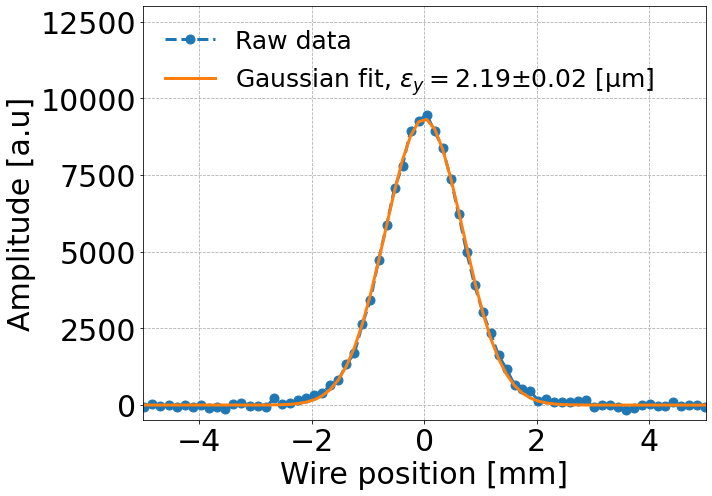
\includegraphics[width=0.6\textwidth]{images/Ch5/SPS.BWS.41677.V_ROT_2018-09-05 15_45_01.33500_raw_and_fit.png}
       \caption{Vertical beam profile obtained from the BWS.41677.V instrument. The measured data points (light blue) are fitted with a four parameter gaussian (orange) to obtain the beam size. The calculated emittance and its uncertainty are also shown.}
       \label{fig:WS_example_V_profile}
\end{figure}
   
%\normalsize{\textbf{Computing the normalised beam emittance}}\\
\subsubsection*{Computing the normalised beam emittance}
The formula for computing the normalised beam emittance from the beam size, $\sigma_u$ is given by:
\begin{equation}\label{eq:emittance_from_WS}
   \centering
   \epsilon_u = \frac{\sigma_u^2}{\beta_{u, WS}} \betarel \gammarel ,
\end{equation}
where $\sigma_u$ is the rms beam size, $\beta_{u, WS}$ the beta function at the Wire Scanner location and $\betarel, \gammarel$ the relativistic parameters. Note that $u=x,y$ is the index that respectively corresponds to the horizontal and vertical plane.

Assuming that the relativistic parameters are free of error, the uncertainty of the computed emittance, $\Delta \epsilon_u$, depends on the uncertainty of the measured beam size, $\Delta \sigma_u$ and of the beta function at the location of the Wire Scanner, $\Delta \beta_{u, WS}$, as follows:
\begin{equation}\label{eq:emittance_from_WS_uncertainty}
   \centering
   \Delta \epsilon_u = \sqrt{\left ( \frac{\partial \epsilon_u}{\partial \sigma_u}\right )^2 \Delta \sigma_u^2 + \left ( \frac{\partial \epsilon_u}{\partial \beta_{u, WS}} \right )^2 \Delta \beta_{u, WS}^2} = \epsilon_u  \sqrt{\left ( \frac{2 \Delta \sigma_u}{\sigma_u}\right )^2 + \left ( \frac{ \Delta \beta_{u, WS}}{\beta_{u, WS}} \right )^2} .
\end{equation}
% Propagation of uncertainty in paper: /eos/user/n/natriant/Project_thesis/material/Ch4: 1st experimental campaign in SPS/propagation_of_uncertainty_emittance.pdf

For the computation of the emittance values from the $\CC$ experiment of 2018, the following points were considered. First, in the 2018 SPS operational configuration, the dispersion was small at the Wire Scanner location and thus its contribution to the beam size was considered to be negligible \footnote{BWS.51995.H location in 2018 was located at a low-dispersion region $D_x < 0.5$\,m~\cite{Roncarolo:1481835}. At 270\,GeV, the energy spread, $\delta$, is of the order of $\mathrm{10^{-4}}$. Thus, from Eq.~\eqref{eq:emit_from_beam_size} the horizontal normalised emittance from the dispersion is expected at the order of $\mathrm{9\times 10^{-3} \ \mu m}$. Comparing to the observed beam size during the CC tests of a few microns the dispersion is negligible and hence it will not be considered in the following. This is also confirmed by past studies~\cite{Roncarolo:1481835}. The measured vertical dispersion has similar value with the horizontal~\cite{Hannes_personal_communication} hence its contribution in the measured vertical emittance will also not be considered in the folllowing}. Moreover, for the studies at 270\,GeV beam energy, $\betarel \gammarel$ equals 287.8 and the beta functions were 81.5\,m and 62.96\,m at the locations of the horizontal and vertical Wire Scanner respectively. Last, the uncertainty on the beta functions at the location of the Wire Scanner, $\Delta \beta_{u, WS}$, is 5$\%$ in both planes, which represents the rms beta-beating in the SPS~\cite{SPS-beta-beating-Rogelio}.


% Note 1: Computations on the paper from dispersive contribution:/eos/user/n/natriant/Project_thesis/material/Ch5: Experimental studies 2018/dispersive_contribution_at_bws_h.pdf
% Note 2: Information on the optics of the WS for the 2018 experiment in the following link from lee: https://docs.google.com/document/d/1kpqnNSXJv7Ro7iQ6OtxvnT4EUOSfYEWxjqUxqEZVIG0/edit or /eos/user/n/natriant/Project_thesis/SPS optics/Crab Cavity Location.pdf. In the table of page 2 it is mentioned that for the WS BWSA.51995 the device name was Wire Scanner 519. 
% Note 3: From Federicos' thesis in p.114 it is mentioned that the  Wire Scanner 519 is located in a low dispersion region < 0.5 m.
% Note 4: In Federic's thesis in Fig.(8.11) it can be seen that the dependnece on the rms momentum spread for the Wire Scanner 517 which is also located in a low dispersion region is almost negligble (pink line). These studies are for 26 GeV so for 270 GeV the dependence on the momentum spread is even smaller.
% Note 5: Link to Federicos thesis: https://cds.cern.ch/record/1481835/files/CERN-THESIS-2005-082.pdf


\textbf{Further considerations}\\
It is worth noting here that during each measurement with the Wire Scanner the beam profile is actually acquired twice as the wire crosses the beam in the forward direction (IN scan) and then in the reverse direction (OUT scan). For the 2018 measurements the emittance values obtained from IN and OUT scans, $\epsilon_\mathrm{IN} \pm \Delta \epsilon_\mathrm{IN}$ and $\epsilon_\mathrm{OUT} \pm \Delta \epsilon_\mathrm{OUT}$, were found to be very similar. In the analysis of the 2018 measurements, the average emittance from the two scans, $\epsilon_\mathrm{avg} = \langle \epsilon_\mathrm{IN}, \epsilon_\mathrm{OUT}\rangle$, is used. The uncertainty in the average, $\Delta \epsilon_\mathrm{avg, 1}$, is given by~\cite{uncertainty_in_the_mean}: 
\begin{equation}\label{eq:uncertainty_mean_ws}
   \Delta \epsilon_\mathrm{avg, 1} = \frac{\mid \epsilon_\mathrm{IN} - \epsilon_\mathrm{OUT} \mid}{2 \sqrt{2}}.
\end{equation}
The propagated uncertainty from the measurement errors, $\Delta \epsilon_\mathrm{IN}$ and $\Delta \epsilon_\mathrm{OUT}$, is given by:
\begin{equation}\label{eq:propagated_uncertainty_ws}
   \Delta \epsilon_\mathrm{avg, 2} = \frac{1}{2}\sqrt{ \Delta \epsilon_\mathrm{IN}^2 + \Delta \epsilon_\mathrm{OUT}^2}.
\end{equation}
Assuming that $\Delta \epsilon_\mathrm{avg, 1}$ and $\Delta \epsilon_\mathrm{avg, 2}$ are independent, the combined uncertainty in the average, $\Delta \epsilon_\mathrm{avg}$, is given by:

\begin{equation}\label{eq:combined_uncertainty_ws}
   \Delta \epsilon_\mathrm{avg} = \sqrt{\Delta \epsilon_\mathrm{avg, 1} ^2 + \Delta \epsilon_\mathrm{avg, 2} ^2}.
\end{equation}

Finally, some emittance increase is expected during each wire scan, due to multiple Coulomb scattering. This effect has been extensively studied in~\cite{Roncarolo:1481835}. For the rotational SPS Wire Scanners and the energy of 270\,GeV, at which the $\CC$ experiments were performed the expected emittance growth from the Wire Scanner is expected to be a few nanometeres per scan in both transverse planes~\cite{Roncarolo:1481835} which is very small with respect to the emittance values of a few micrometers. Nevertheless, a conservative number of scans were carried out, $\sim$20 scans per bunch and per plane during $\sim$1 hour, in order to minimise the contribution from this effect.
% Note 1: Link to federico's thesis: https://cds.cern.ch/record/1481835/files/CERN-THESIS-2005-082.pdf
% Note 2: Table 5.1 0.0% for 450 GeV, 0.2% per scan
% Note 3: Also "p.70 The measurements show an emittance growth of 43.5±11.8 nm per scan, which is best approximated by prediction 3)." . I think this is for 26 GeV, for 270 GeV the blow up would be even smaller.

\subsection{Experimental results}\label{sec:MD5_overview}
In this section, an overview of the emittance growth measurements is presented. Figure~\ref{fig:MD5_overview_x_y} displays the bunch by bunch transverse emittance evolution throught the total duration of the experiment. The three different coasts are distinguished in this plot with the blue dashed vertical lines. The values of the effective phase noise are also displayed (see Table~\ref{tab:noise_settings_2018}), while the moments when the noise level changed are shown with the grey vertical lines. The four different colors (blue, orange, red, green) correspond to the four different bunches. For the bunches the notation "bunch $N$" will be used, where $N=\{1,2,3,4\}$ according to their position in the bunch train. The errorbars of the emittance values correspond to the uncertainty computed using Eq.~\ref{eq:combined_uncertainty_ws}. However, as they are very small compared to the scale of the plots they are barely visible. Last, the emittance growth rates, $d\epsilon_u /dt$, for each setting and for each bunch are displayed at the bottom of each plot along with their uncertainties. The growth rates are obtained following the standard procedure of weighted least squares fitting (see Appendix~\ref{app:non_linear_fitting}). In particular, the measured beam profiles from each scan are fitted with the following polynomial:
% fit with numpy polyfit
\begin{equation}\label{eq:polynimial_for_linear_fit}
   p(x) = c_0 + c_1 \times t
\end{equation}
where $t$ is the time in seconds, $c_0$ is called the intercept and shows where the line estimated from the fit crosses the y-axis, and $c_1$ determines the slope of the line estimated from the fit.  In the case of the emittance growth measurements, $c_0$ corresponds to the initial value of the emittance in meters, while $c_1$ is the growth rate, $d\epsilon_u /dt$, in meters per second. The uncertainties of the growth rates correspond to the error of the fit (see Appendix~\ref{app:non_linear_fitting}).
%$d\epsilon_u /dt$ the growth rate in meters per second and $c_0$ the constant offset in meters. The uncertainties of the growth rates correspond to the error of the fit (see Appendix~\ref{app:non_linear_fitting}). 

% Analysis and figures: /eos/user/n/natriant/2018/CC_MD_2018_summary/emitGrowth_ws
% Merge png online free: https://products.aspose.app/pdf/merger/png-to-png
\begin{sidewaysfigure}
   \centering
   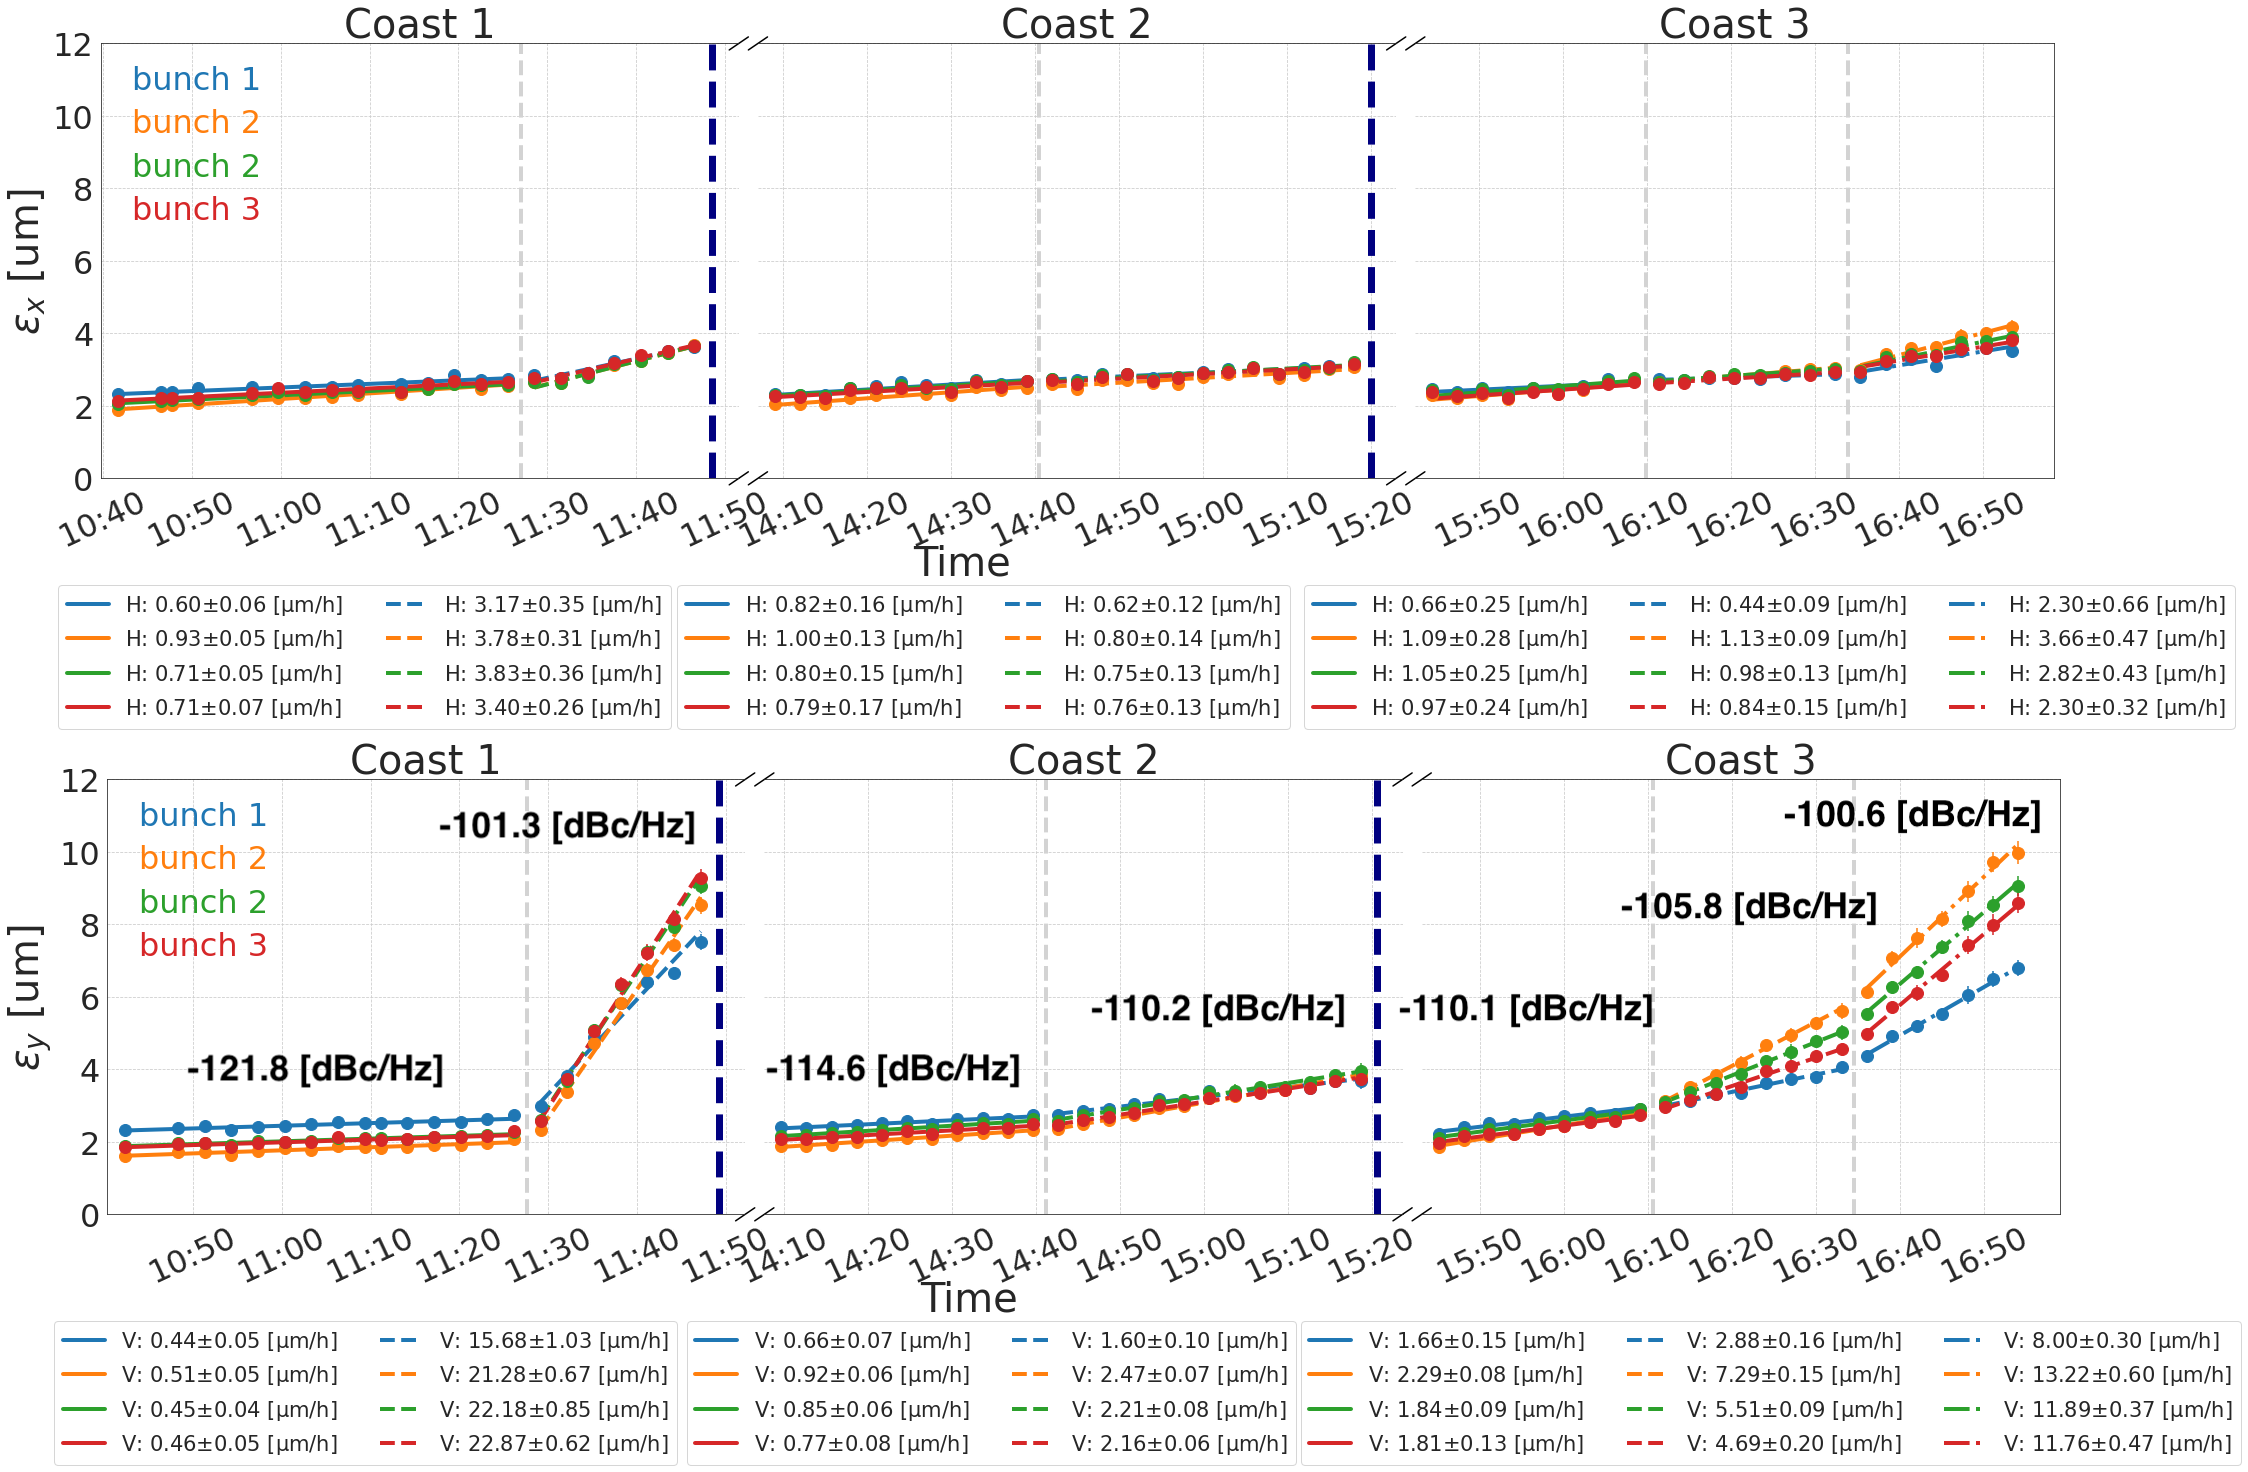
\includegraphics[width=1.0\textwidth]{images/Ch5/MD5_overview_x_y.png}
   \caption{Bunch by bunch horizontal (top) and vertical (bottom) emittance evolution during the experiment on September, 15, 2018. The four different colors indicate the different bunches. The different applied noise levels are also shown while the moments when the noise level changed are inficated with the grey vertical dashed lines. The emittance growth rates along with their uncertainties for the seven different noise settings are displayed at the legend at the bottom of the plots.}
   \label{fig:MD5_overview_x_y}
\end{sidewaysfigure}
   
\textbf{First observations and comments}\\
Figure~\ref{fig:MD5_overview_x_y} demonstrates a clear emittance growth in the vertical plane which is expected due to the vertical $\CC$. \textcolor{red}{The following sentences need to be revised}. However, the $\CC$ noise is observed to induce growth also in the horizontal emittance as a result of residual coupling in the machine. Thus, the total emittance growth given by $d\epsilon_x/dt + d\epsilon_y/dt$ should be considered in the following. That was confirmed by PyHEADTAIL simulations~\cite{Baudrenghien_HL-LHC19v6} in the presence of $\CC$ RF noise and transverse coupling. 

% Maybe re-write:  However, emittance growth is also observed in the horizontal plane as will which seems to be a result of residual coupling in the machine.\footnote{the betatron coupling in sps is small, $\sim$ 10^{-3}~\cite{hannes personal communication} but not zero}. The total emittance growth given by $d\epsilon_x/dt + d\epsilon_y/dt$ will be considered in the following... --> we need to think  That was confirmed by PyHEADTAIL simulations~\cite{Baudrenghien_HL-LHC19v6} in the presence of $\CC$ RF noise and transverse coupling. 


Furthermore, both the phase and amplitude noise levels for Coast$1$-Setting$1$ were found to be below the noise floor of the $\CC$. Therefore, the transverse emittance growth observed during that case is a result of other sources (natural emittance growth, see Section~\ref{sec:preparatory_studies_for_2018_MD} ) and will be considered as the background growth rate in the analysis below. 

\textbf{Summary plot}\\
Figure~\ref{fig:MD5_summary_plot} provides a clearer view of the measurements presented in Fig.~\ref{fig:MD5_overview_x_y}. It displays the measured emittance growth rates for each one of the four bunches for the different levels of injected noise. The horizontal error bars correspond to the uncertainty of the effective phase noise (see Section~\ref{sec:injected_RF_noise}) while the veritcal errror bars correspond to the uncertainty of the total transverse emittance growth calculated from the uncertainties of the horizontal and vertical growth rates following the standard procedure of the propagation of the uncertainty (Appendix~\ref{app:uncertainty_propagation}).

\begin{figure}[!h]
   \centering         
   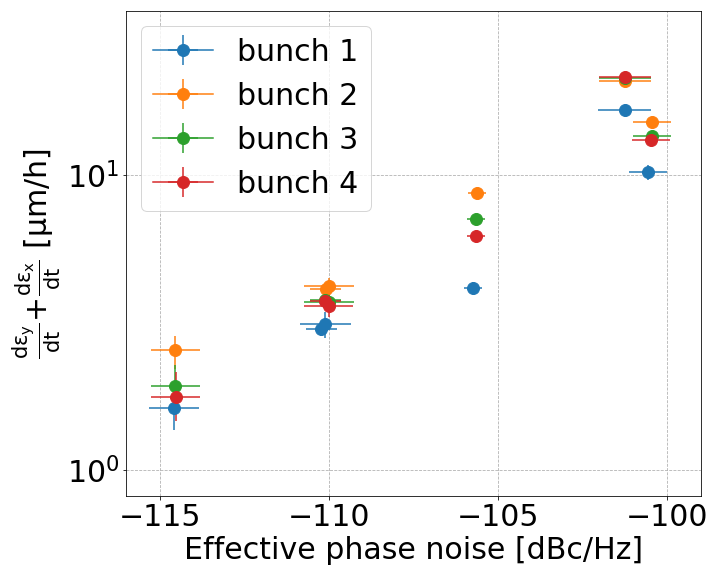
\includegraphics[width=0.6\textwidth]{images/Ch5/MD5_summary_plot_no_backg_subtraction.png}
       \caption{Summary plot of the emittance growth study with CC noise in 2018. The transverse emittance growth rate, for the four bunches, is shown as a function of the different levels of applied noise.}
       \label{fig:MD5_summary_plot}
\end{figure}

From the plot it becomes clear that the measured emittance growth was different for the four different bunches. Furthermore, the first bunch (blue) had systematically the smallest growth rate.

An attempt to understand these observations will be presented in the following section, based on a possible correlation between the transverse emittance growth and the beam evolution in the longitudinal plane.

\section{Bunch length and intensity measurements}\label{sec:bunch_length_intensity_meas_2018}
The measurements of the bunch length and intensity that took place in parallel with the emittance growth measurements are presented in this section. The goal is to get a more complete insight of the experimental conditions and possibly explain the different emittance growth rates observed for the four bunches which was discussed in the previous section. Initially, a short introduction on the instruments used for the measurements is provided. After that, the evolution of the longitudinal plane and of the intensity is analysed and discussed.

\subsection{ABWLM and Wall Current Monitor}\label{sec:ABWLM_WallCurrentMonitor}
The bunch length was measured with two different instruments the ABWLM\footnote{(A for RF, B for Beam, W for Wideband, L for Longitudinal, M for Measurement)}~\cite{ABWLM} and the Wall Current Monitor~\cite{Papotti:1124099}. Both ABWLM and Wall Current Monitor acquire the longitudinal bunch profiles, while ABWLM is much faster than the Wall Current Monitor. %I concluded this from the data. If I need to give specific values I will remove it.
In the ABWLM case the bunch length is obtained by performing a gaussian fit on the acquired profiles. Only the calculated bunch length values are available but not the profiles themselves. For the case of the Wall Current Monitor the bunch length is estimated by computing the full width half maximum of the profiles and then using it to estimate the standard deviation of a gaussian distribution. The longitudinal profiles and the calculated bunch lengths are available for each acquisition. Furthermore, the Wall Current Monitor provides additional information on the relative bunch position with respect to the center of the RF bucket, which will also be used in the following analysis. No further details on the operation of these instruments are discussed here as the offline analysis was not performed by the author. % bunch position not very clear.
% longitudinal profiles for the ABLWM don't exist.

The intensity values obtained from the ABWLM and the Wall Current Monitor are obtained by integration of the longitudinal bunch profiles. Since there is no available calibration for this procedure the measured intensity cannot be expressed in protons per bunch. To this end, the intensity evolution is presented normalised with the intial intensity value (see Fig.~\ref{fig:MD5_overview_intensity}). 

\subsection{Bunch length measurements}\label{subsec:bunch_length_meas_2018}
The bunch length measurements that took place during the $\CC$ noise induced emittance growth studies are shown in the bottom plot in Fig.~\ref{fig:MD5_overview_x_y_sigma_t}. The small markers correspond to the data acquired with the ABWLM while the bigger markers correspond to the data acquired with the Wall Current Monitor. The two upper plots contain the transverse emittance growth as discussed in Section~\ref{sec:MD5_overview}. This is for easier comparison of the beam evolution in the transverse and in the longitudinal plane. The color code corresponds to the four different bunches.

% Script for plotting: /eos/user/n/natriant/2018/CC_MD_2018_summary/ABWLM/job001_abwlm_bunch_length_analysis_plot_overview.ipynb
% Merging with https://photo333.com/merge-png.php
\begin{sidewaysfigure}
   \centering
   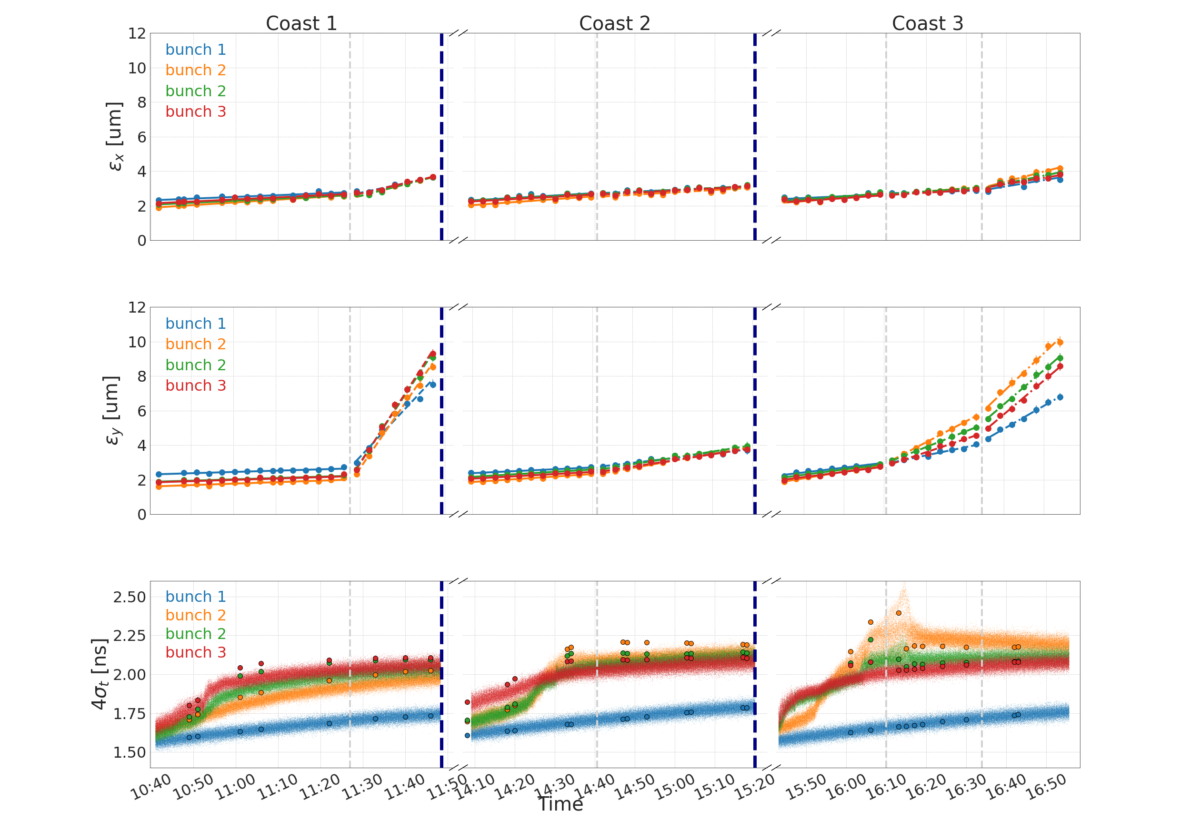
\includegraphics[width=1.0\textwidth]{images/Ch5/MD5_overview_x_no_legendMD5_overview_y_no_legendMD5_overview_4sigma_t_no_title_with_wall_current_monitor.png}
   \caption{Evolution of the beam in transverse and longitudinal planes during the CC noise induced emittance growth experiment. Top: Horizontal emittance growth measured with the SPS Wire Scanners. Middle: Vertical emittance growt measured with the SPS Wire Scanner. Bottom: Bunch length evolution measured with the ABWLM (small markers) and the Wall Current Monitor (bigger markers).}
   \label{fig:MD5_overview_x_y_sigma_t}
\end{sidewaysfigure}
% dont mention about the scaling with the wall current monitor, subtracted offset: -0.18 ns.
% UPDATE 24March:20222. The scaling factor is actually 1/1.11 but I am not gonna correct it now. Is more or less the same. However, if you update the plot again, fix it. 

Four main observations can be made. First, the plot demonstrates a very good agreement between the ABLWM and the Wall Current monitor. Second, an approximately bunch length increase of $\sim$9\,$\%$/h is observed for bunch 1 (blue) in all the three coasts. This rate, which is computed from the ABWLM data, is similar to the blow-up observed in the SPS for similar machine conditions~\cite{Alekou_CC_coast_prep_2016}. Third, the bunch length increase for the last three bunches (2, 3, and 4) is larger than the increase for bunch 1. However, bunches 2, 3, and 4 seem to be longitudinally unstable as sudden jumps appear in their bunch length evolution and this could explain the faster bunch length increase. Last, no correlation is observed between the bunch length evolution and the change of noise level. In order to validate that bunches 2, 3, and 4 are unstable, the longitudinal profiles acquired with the Wall Current Monitor are studied in the next paragraph. 
%cmpt bunch length increase for bunch 1 in units of %/h.

\subsection{Longitunal profile measurements}\label{subsec:long_profiles_meas_2018}
Two example longitudinal profile acquisitions from the Wall Current Monitor are discussed here as they can provide further insight on the sudden jumps observed in the bunch length values for bunches 2, 3, and 4. The selected acquisitions correspond to the moments where the sudden jumps are performed in the second and third coast and are shown in Fig~\ref{fig:long_profiles_and_rel_bunch_position_2018}. The relative bunch position with respect to the center of the RF bucket of each bunch for an acquisition period of 7\,ms is also illustrated in the bottom plots of Fig.~\ref{fig:long_profiles_and_rel_bunch_position_2018} for completeness. 


\begin{figure}[!ht]
   \centering
   \begin{subfigure}[t]{0.42\textwidth}
       \centering
       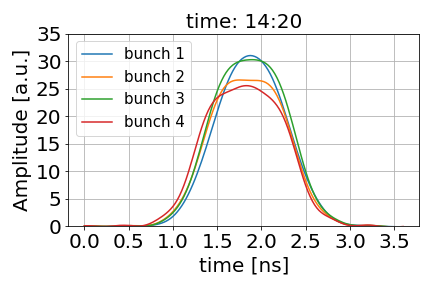
\includegraphics[width=1\textwidth]{./images/Ch5/bunchProfiles_MD_115.png}
       %\caption{Phase noise spectrum measured with a spectrum analyzer E5052B, in units dBc/Hz.}
       %\label{fig:coast1_setting2_a}
   \end{subfigure}
   \hfill
   \begin{subfigure}[t]{0.42\textwidth}
       \centering
       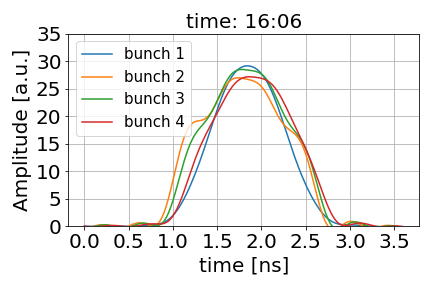
\includegraphics[width=1 \textwidth]{./images/Ch5/bunchProfiles_MD_126.png}
       %\caption{Measured phase noise spectrum in  units rad$^2$/Hz.}
       %\label{fig:coast1_setting2_b}
   \end{subfigure}
   \hfill
   \begin{subfigure}[t]{0.42\textwidth}
       \centering
       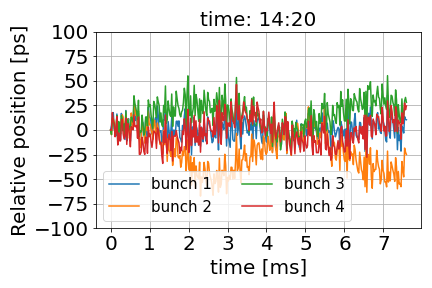
\includegraphics[width=1\textwidth]{./images/Ch5/bunchPosition_MD_115.png}
       %\caption{Linear interpolation of the measured noise spectrum. %sampled every $\Delta f = f_{rev}/N$. Here $f_{rev}$=43.45 [kHz] and N=$10^5$ turns are used.}
       
       %\label{fig:coast1_setting2_c}
   \end{subfigure}
   \hfill
   \begin{subfigure}[t]{0.42\textwidth}
       \centering
       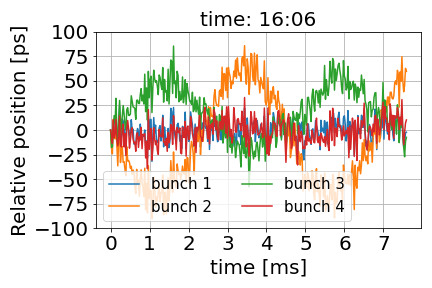
\includegraphics[width=1\textwidth]{./images/Ch5/bunchPosition_MD_126.png}
       %\caption{Positive spectral components of the two-sided power spectrum $S_\phi$.}
       %\label{fig:coast1_setting2_d}
   \end{subfigure}
   \hfill
   \caption{Longitudinal profiles (top) and relative bunch position with respect to the center of the RF bucket (bottom) acquired with the Wall Current Monitor. The acquisitions correspond to the times when the sudden jumps in the bunch length evolution are observed (see Fig.~\ref{fig:MD5_overview_x_y_sigma_t}).}
   \label{fig:long_profiles_and_rel_bunch_position_2018}
\end{figure}
% Each acquisition, last 7 ms? And then we compute the average? Is that right?
% The profiles, are averaged over a period of 7 ms. More details here: https://docs.google.com/presentation/d/1wqgJK7uDFDGoX8gyx2-JhnO8mZT51N1VH1RtNL-jhWA/edit?usp=sharing
% Hannes: The relative bunch position is with respect to the center of the bucket of each bunch, as obtained from the revolution frequency clock I would say. The revolution frequency clock is the system that keeps track of the revolution frequency of the beam

The oscillations of the relative bunch position (bottom) of the bunches 2,3 and 4 (orange, green, and red) indicate that the bunches are longitudinally unstable. This is also reflected in the longitudinal profiles (top) which appear distorted. The reason behind the longitudinally unstable bunches is believed the fact that that the phase loop was sampling only the first bunch
because of the large bunch spacing of 525\,ns~\cite{Argyropoulos_unstable_bunches_2018}. For this reason, the following analysis is focused only on bunch 1, which was not affected by the instability. However, in the next paragraph the intensity measurements for all the four bunches are exceptionally illustrated.

%From Fig.~\ref{fig:long_profiles_and_rel_bunch_position_2018}, it becomes clear that bunches 2,3, and 4 (orange, green, and red) are longitudinally unstable. 
\subsection{Intensity measurements}\label{subsec:intensity_2018_meas}
The bunch by bunch intensity measurements that were performed along the experiment with artificial $\CC$ noise are displayed in Fig.~\ref{fig:MD5_overview_intensity}. In particular the intensity values normalised with the intial value are shown for each bunch. The four different bunches are indicated with the four different colors. The acquisitions from both the ABWLM and the Wall Current Monitor are illustrated with the small and bigger markers respectively.

The following observations can be made. First, there is very good agreement between the measruments from the ABLWM and the Wall Current Monitor. Second, losses of $\sim$2-4\,$\%$/h, computed from the ABLWM acquisitions, are observed for bunch 1 (blue) in all the three coasts. This rate is even smaller than observed in the SPS in coast studies without external noise ($\sim$10\,$\%$/h)~\cite{Alekou_CC_coast_prep_2016}. Last, more significant losses are observed for the longitudinally unstable bunches (bunch 2,3, and 4). However, this is not of concern as the last three bunches will not be included in the following analysis as discussed in the previous paragraph (~\ref{subsec:long_profiles_meas_2018}).

\begin{sidewaysfigure}
   \centering
   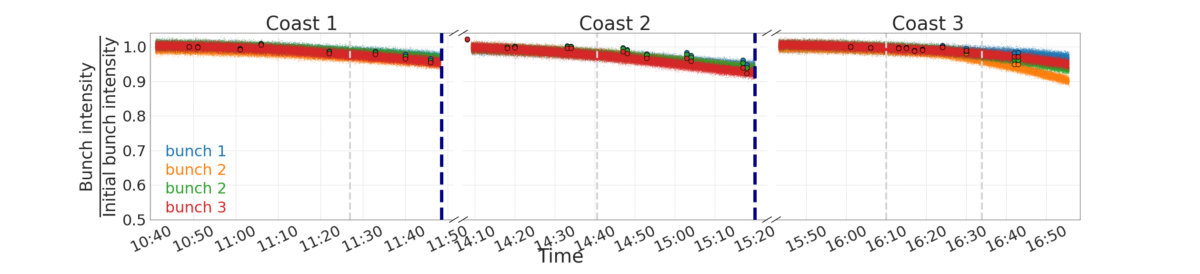
\includegraphics[width=1.0\textwidth]{images/Ch5/MD5_overview_intensity_with_wall_current_monitor.png}
   \caption{Intensity evolution as measured with ABLWM (smaller markers) and with the Wall Current Monitor (bigger markers) during the experiment with CC noise in 2018.}
   \label{fig:MD5_overview_intensity}
\end{sidewaysfigure}
% Scripts: /eos/user/n/natriant/2018/CC_MD_2018_summary/ABWLM/job004_abwlm_bunch_intensity_analysis_plot_overview_with_wall_current_monitor.ipynb
% ABWLM data: /eos/user/n/natriant/2018/CC_MD_2018_summary/ABWLM/output/abwlm_bunch_intensity.pkl
% Wall Current Monitor data: /eos/user/n/natriant/2018/CC_MD_2018_summary/Wall_Current_Monitor/pickled_data_from_2018

\section{Comparison of measured transverse emittance growth with the theoretical predictions}\label{sec:meas_2018_vs_theory}
This section focuses on the main objective of the experiment which was the comparison of the measured transverse emittance growth with the expected values as computed from the Mastoridis--Baudrenghien model introduced in Chapter~\ref{Ch:CC_noise_theory}. As already discussed (Section~\ref{subsec:long_profiles_meas_2018}), the comparison considers only bunch 1 as the other three bunches were found to be longitudinally unstable.

Figure~\ref{fig:MD5_bunch1_theory_vs_meas} compares the the measured (blue) and the theoretically calculated (black) emittance growth rates of bunch 1 for the different noise levels. For the comparison, the background growth rate from other sources (measured during Coast$1$-Setting$1$, as discussed in Section~\ref{sec:emit_growth_meas_2018}) is subtracted from the measured values. In particular the background growth was measured 0.6\,$\mathrm{\mu m}$/h and 0.44\,$\mathrm{\mu m}$/h for the horizontal and veritcal plane respectively. One should keep in mind that background subtraction has practically no impact for high noise levels. Instead, it is significant for small noise levels.


The expected emittance growth due to $\CC$ noise was estimate for all noise settings using Eq.~\eqref{eq:dey_pn}. The growth was computed for the beam energy of 270\,GeV, considering the veritcal beta function at the location of the $\CC$2 of 73.82\,m and the revolution frequency of SPS which is 43.37\,kHz. For each setting, the measured noise power spectral densities (i.e. effective phase noise) and the average bunch length over each observation window were used in the calculation. These values are listed in the first two columns of Table~\ref{tab:MD5_bunch1_results}.

The horizontal error bars, for both measured and calculated growths, correspond to the uncertainty of the effective phase noise values (see Table~\ref{tab:noise_settings_2018}). The vertical error bars for the measured growth are defined as the error of the linear fit on the emittance values (see Section~\ref{sec:emit_growth_meas_2018}). The veritcal error bars on the theoretically calculated rates are computed following the standard procedure of propagation of the uncertainty. It should be mentioned here that only the uncertainties on the effective phase noise ($\sim$ 13\% on average for bunch 1) are included in the error propagation. The beam energy and the revolution frequency are assumed to be free of error, while the uncertainties of the rest of the parameters: bunch length, $\CC$ votlage and beta function ($\sim 2 \%, \ 0.01 \%$, and $5 \%$ respectively) are not included as they are much smaller than those of the noise.


% 1. Compute % uncertainty on the bunch length: /eos/user/n/natriant/2018/CC_MD_2018_summary/ABWLM/job0006_cmpt_averaged_bunch_length_and_uncertainty_for_each_setting_save2pickle.ipynb
% 2. Uncertainty on the beta function is 5% from beta beating. 
% 3. Compute uncertainty on the PSD --> in rad^2/Hz NOT in dBc/Hz as this is the form that it enters the Eq.(3.2).
% 4. Uncertainty on the V_CC is 0.01/0.98*100 = 0.01%
% 5. Compute the theoretically growth rates: /eos/user/n/natriant/2018/CC_MD_2018_summary/cmpt_emit_growth_theoretical_model/job001_cmpt_theoretical_emit_growth_MD5_2018.ipynb
% Compute the unertainty on the theoretical growth rates: /eos/user/n/natriant/2018/CC_MD_2018_summary/cmpt_emit_growth_theoretical_model/job003_cmpt_uncertainty_on_theoretical_emit_grwoth_MD_2018.ipynb and the computation is done accordind to the notes in the measured_psd directory. In general the procedure is the same with computing the uncertainty of the measured effective noise.


\begin{figure}[!h]
   \centering         
   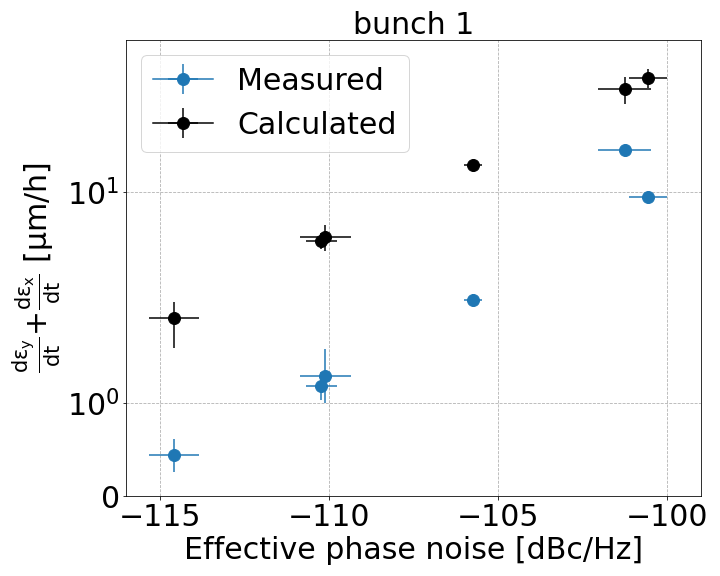
\includegraphics[width=0.6\textwidth]{images/Ch5/MD5_summary_bunch1_backg_subtracted_vs_theory.png}
       \caption{Summary plot of the emittance growth study with CC noise in 2018 focused on bunch 1 only. The measured emittance growth rate (blue) and the expected growths from the theoretical model (black) are shown as a function of the different levels of applied noise.}
       \label{fig:MD5_bunch1_theory_vs_meas}
\end{figure}


From Fig.~\ref{fig:MD5_bunch1_theory_vs_meas} it becomes evident that the theory systematically overestimates the measured growth rates. The averaged discrepancy over all noise levels is a factor of 4: numerical values are given in Table~\ref{tab:MD5_bunch1_results}. The measurements seem to go in the good direction but actually they show that there is a significant uncertainty on the predictions of the theoretical model. The accuracy of the model is essential for defining the specifications for the design of the HL-LHC CC LLRF. Therefore, understanding the reason behind the observed descrepancy with the measurements which would also allow to decide if the reduction of the factor 4 can be porpagated for the HL-LHC predictions is fundamental. The studies performed to explain the discrepancy will be described in the following chapters.

% Compute average bunch length: /eos/user/n/natriant/2018/CC_MD_2018_summary/ABWLM/job0006_cmpt_averaged_bunch_length_and_uncertainty_for_each_setting_save2pickle.ipynb
% Find measured and calculated growth rates: /eos/user/n/natriant/2018/CC_MD_2018_summary/emitGrowth_ws/job006_plot_bunch_1_theory_vs_measurements.ipynb

\begin{table}[!hbt]
	\centering
   \caption{Comparison between the measured and the calculated transverse emittance growth rates for bunch 1 for the different noise levels, and average bunch length for each case.}
	\begin{tabu} to \textwidth { X[c,m] X[c,m] X[c,m] X[c,m]}
		&&& \\[-6mm]
		\toprule \toprule
		\multicolumn{1}{c}{$\mathbf{10\,\boldsymbol{\log}_{10} \mathcal{L}(f)}$} &
		\multicolumn{1}{c}{$\mathbf{\boldsymbol{\langle \sigma_\phi \rangle}}$} & \multicolumn{2}{c}{\textbf{Growth rate [}$\mathbf{\boldsymbol{\mu}}$\textbf{m/h]}}  \\
		%\bottomrule
      \multicolumn{1}{c}{\textbf{[dBc/Hz]}} & \multicolumn{1}{c}{\textbf{[rad]}} & \multicolumn{1}{c}{\textbf{Measured}} & 	\multicolumn{1}{c}{\textbf{Calculated}} \\
      \midrule
      \multicolumn{1}{c}{-114.6}  & \multicolumn{1}{c}{1.05} & \multicolumn{1}{c}{0.44} & \multicolumn{1}{c}{1.9} \\
      
      \multicolumn{1}{c}{-110.2}  & \multicolumn{1}{c}{1.10} & \multicolumn{1}{c}{1.18} & \multicolumn{1}{c}{5.10} \\

      \multicolumn{1}{c}{-110.1}  & \multicolumn{1}{c}{1.03} & \multicolumn{1}{c}{1.28} & \multicolumn{1}{c}{5.38} \\

      \multicolumn{1}{c}{-105.8}  & \multicolumn{1}{c}{1.06} & \multicolumn{1}{c}{2.28} & \multicolumn{1}{c}{14.50} \\ 

      \multicolumn{1}{c}{-101.3}  & \multicolumn{1}{c}{1.08} & \multicolumn{1}{c}{17.81} & \multicolumn{1}{c}{40.55} \\

      \multicolumn{1}{c}{-100.6} & \multicolumn{1}{c}{1.09} & \multicolumn{1}{c}{47.42} & \multicolumn{1}{c}{9.26}\\
      \arrayrulecolor{black}\bottomrule
	\end{tabu}
   \label{tab:MD5_bunch1_results}
\end{table}


\section{Conclusions and outlook}\label{sec:MD2018_conclusions}
The objective of the first experimental campaign with $\CC$ noise in the SPS was to benchmark the available theoretical model which predicts the noise induced transverse emittance growth against measruments. For this reason, a dedicated experiment took place in the SPS in September of 2018, with different leves of artificial noise injected in the $\CC$ RF system. Four bunches circulated in the machine for long periods of time and their emittance evolution was recorded to be compared with the theoretical predictions.


The experiment demonstrated that the transverse emittance of all the four bunches increased for stronger noise. However, during the analysis it was found that only the first bunch of the train was stable in the longitudinal plane. For this reason, only the data from the first bunch were used for the comparison with the theoretically calculated emittance growth rates. The comparison showed that the theoretically overestimates the measurements by a significant factor of 4. The reason behind this discrepancy needs to be understood as the predictions of the theoretical model will be used to define limits and acceptable noise levels for the HL-LHC $\CC$s. Therefore, the next chapters focus on explaining the observed discrepancy.
